\documentclass[11pt,reqno, usenames]{report}
\renewcommand{\rmdefault}{ppl}  % Skifter til Times New Roman
\usepackage[a4paper, hmargin=2cm, tmargin=2.5cm, bmargin=3cm]{geometry}

% \newtheorem{theorem}{Teorem}[section]
% \newtheorem{lemma}{Lemma}[section]
\usepackage{amsthm}
\usepackage{enumitem}


%%%%%%%%%%%%%%%%%%%%% Sætnings design

\usepackage[listings]{tcolorbox} 
\tcbuselibrary{listings,theorems}

\definecolor{codeblue1}{rgb}{0.404, 0.576, 0.839}


% \newtcbtheorem[use counter=theorem, number within=section]{mytheo}{Sætning}%
% {colback=codeblue!5,              % light blue background
%  colbacktitle=codeblue1,           % strong blue title bar
%  colframe=codeblue1,               % blue border
%  coltitle=white,                  % white text in the title
%  fonttitle=\bfseries,             % bold title font
%  title prefix=, title suffix=:,   % format of "Sætning 1:"
%  title after break = \textit{(fortsat)},
%  breakable,
%  enhanced}
% {th}

\tcbuselibrary{listings,theorems}

\newtcbtheorem{mytheo}{Sætning}%
{colback=codeblue!5,colframe=codeblue,fonttitle=\bfseries}{th}


%%%%%%% tables formatting %%%%%%
\usepackage[usenames,dvipsnames]{xcolor}
\usepackage{tcolorbox}
\usepackage{tabularx}
\usepackage{array}
\usepackage{colortbl}
\tcbuselibrary{skins}
\newcolumntype{Y}{>{\raggedleft\arraybackslash}X}
\newcolumntype{C}{>{\centering\arraybackslash}X} % Centered column type


\tcbset{tab1/.style={fonttitle=\bfseries\large,fontupper=\normalsize\sffamily,
colback=codeblue!10!white,colframe=codeblue!35!black,colbacktitle=codeblue!35!white,
coltitle=white,center title,freelance,frame code={
\foreach \n in {north east,north west,south east,south west}
{\path [fill=codeblue!75!black] (interior.\n) circle (3mm); };},}}


\tcbset{tab2/.style={enhanced,fonttitle=\bfseries,fontupper=\normalsize,
colback=codeblue!10!white,colframe=codeblue!40!black,colbacktitle=codeblue!90!white,
coltitle=white,center title}}

\usepackage{booktabs}
\usepackage{caption}
\usepackage{amsmath}
\usepackage{siunitx}
\usepackage{multirow}
\usepackage{threeparttable}
\usepackage{xcolor}
\usepackage{colortbl}
%\usepackage{cellspace}
\usepackage{rotating}
% \setlength\cellspacetoplimit{3pt}
% \setlength\cellspacebottomlimit{3pt}

\usepackage{etoolbox}
\makeatletter
\patchcmd{\chapter}{\if@openright\cleardoublepage\else\clearpage\fi}{}{}{}
\makeatother


% Define colors
\definecolor{teal}{RGB}{0, 128, 128}
\definecolor{lightgray}{RGB}{230, 230, 230}

% \usepackage{amsmath}
% \usepackage{amssymb}
\usepackage{float}
\usepackage{wrapfig}
\usepackage[utf8]{inputenc}
\usepackage[table]{xcolor}
\usepackage{tikz}
\usepackage{pgfplots}
\pgfplotsset{compat=1.18}
\usepackage[toc,page]{appendix}
\usepackage{placeins}
\usepackage{fancyhdr}
\usepackage{titlesec}
\usepackage{bm}
\usepackage{setspace}
\usepackage{booktabs}
\usepackage{caption}
\usepackage{booktabs}
\usepackage[utf8]{inputenc}

\usepackage{float} % for [H]
\usepackage[style=authoryear, backend=biber, maxnames=2, uniquelist=false]{biblatex}
\addbibresource{Afsnit/Litteratur.bib}
\DeclareCiteCommand{\citeyearpar}
  {\usebibmacro{prenote}\bibopenparen}
  {\bibhyperref{\printdate}}
  {\multicitedelim}
  {\bibcloseparen\usebibmacro{postnote}}
  
\pagestyle{fancy}
\definecolor{cbsblue}{rgb}{0.788, 0.878, 0.961}
\usepackage{subcaption}
\usepackage{graphicx}
\usepackage{booktabs}
\usepackage{amsfonts}
\usepackage{booktabs}
\usepackage{array}
\usepackage{tabularx}



\usepackage{pgfplots}
\usepackage{booktabs}
\usepackage{threeparttablex}
\usepackage{caption}
\pgfplotsset{compat=1.18}

\usepackage{threeparttable}
%%%%%%%%%%%% Linjeafstand %%%%%%%%%%%%
\onehalfspacing  % 1.5 linjeafstand
%\doublespacing  % 2.0 linjeafstand
%\singlespacing  % Normal linjeafstand (standard)


\usepackage[]{cbs-forside} %CBS forside
\title{Incentives, Costs, and Attrition: A Survival Analysis of Rider Abandonment in Grand Tour Cycling (2010--2025)}
\undertitelI{Student number: S160645}
\vejleder{Field of study: Cand.merc.mat.}
\opgave{} 
\dato{}
\normalsider{}



%%%%%%%%%%%%%%%%%%%%%%%%%%%%%%%%%%%%%%%%%%%%%%%%%%%%%%%%%%%%%%%%%%%%%%%%%%%%%%%%%

\usepackage{hyperref}
\setlength{\abovedisplayskip}{0pt}
\setlength{\belowdisplayskip}{0pt}
\setlength{\abovedisplayshortskip}{0pt}
\setlength{\belowdisplayshortskip}{0pt}
\setlength{\parindent}{0pt}


%%%%%%%%%%%% Sidehoved %%%%%%%%%%%%
\fancyhf{} % Rens standard sidehoved/fod
\fancyhead[L]{S160645} % Venstre sidehoved
\fancyhead[C]{Household behaviour over the lifecycle} % Centreret sidehoved
\renewcommand{\headrulewidth}{0.1pt} % Linje under sidehovedet
\setlength{\headsep}{15mm}  %Afstand mellem sidehoved og overskrift

\fancyfoot[C]{\thepage\ of \pageref{LastPage}} % Sidetalformat: 2 af 64




%%%%%%%%%%%% Kommandoer og hotkeys  %%%%%%%%%%%%
\definecolor{nicered}{rgb}{1, 0, 0}
\newcommand\Red[1]{\textcolor{nicered}{#1}}
	%%%Bogstavlignende symboler
		\newcommand{\mR}{\mathbb{R}}
		\newcommand{\mZ}{\mathbb{Z}}
		\newcommand{\mN}{\mathbb{N}}
		\newcommand{\mQ}{\mathbb{Q}}
		\newcommand{\mC}{\mathbb{C}}
		
		\newcommand{\cA}{\mathcal{A}}
		\newcommand{\cB}{\mathcal{B}}
		\newcommand{\cC}{\mathcal{C}}
		\newcommand{\cD}{\mathcal{D}}
		\newcommand{\cE}{\mathcal{E}}
		\newcommand{\cF}{\mathcal{F}}
		\newcommand{\cG}{\mathcal{G}}
		\newcommand{\cH}{\mathcal{H}}
		\newcommand{\cP}{\mathcal{P}}
		\newcommand{\cN}{\mathcal{N}}
        \newcommand{\mBF}{\mathbf{}}

	%%%Grænseværdi-shorthands
		\newcommand{\limn}{\lim_{n\rightarrow \infty}}
		\newcommand{\forn}{\hspace{10pt} \text{for} \hspace{6pt} n \rightarrow \infty}
		\newcommand{\konv}[1]{\overset{#1}{\rightarrow}}




\setlength\bibitemsep{0.8em}

% --- Make section numbering independent of chapter (report -> article-like) ---
\setcounter{secnumdepth}{3}
\setcounter{tocdepth}{3}

\makeatletter
% Numbering format: 1, 1.1, 1.1.1 (no chapter prefix)
\renewcommand{\thesection}{\arabic{section}}
\renewcommand{\thesubsection}{\thesection.\arabic{subsection}}
\renewcommand{\thesubsubsection}{\thesubsection.\arabic{subsubsection}}

% Reset section counters if a chapter ever appears (harmless if you never use \chapter)
\@addtoreset{section}{chapter}
\@addtoreset{subsection}{chapter}
\@addtoreset{subsubsection}{chapter}

% Fix hyperref anchors to match
\renewcommand{\theHsection}{\arabic{section}}
\renewcommand{\theHsubsection}{\thesection.\arabic{subsection}}
\renewcommand{\theHsubsubsection}{\thesubsection.\arabic{subsubsection}}
\makeatother

% eksempel -> \Red{Noget i farver} 
%%%%%%%%%%%% Dokument begyndelse %%%%%%%%%%%%
\begin{document}

%%%Forside
\maketitle

%%% Fixer side hoved og sidetal
\clearpage
\pagestyle{fancy}
\setcounter{page}{1}


%%% Fordi vi har chapter så laver de nikke sider der, det fikser vi med dette
\makeatletter
\let\ps@plain\ps@fancy
\makeatother

%%%%%%%%%%%% Indhold %%%%%%%%%%%%

\tableofcontents

\newpage

% --------------------------------------------------
% 1. INTRODUCTION
% --------------------------------------------------
\section{Introduction}

In May 2013, Bradley Wiggins, the reigning Tour de France champion, abandoned the Giro d'Italia after just seven stages. His departure was not simply a sporting story. Team Sky had built its entire Giro campaign around Wiggins, allocating domestiques, logistics, and media attention to support his General Classification (GC) bid. When he climbed off his bike, the team lost its primary investment for the race, sponsors lost three weeks of planned television exposure, and Wiggins himself saw his market value as a Grand Tour rider come under scrutiny. Episodes like this raise a question at the intersection of sports and economics: what determines whether a rider continues or abandons a Grand Tour?

This paper treats rider abandonment as an economic decision. At every stage of a Grand Tour, the rider and his team face a choice under uncertainty: continue and bear the physical and strategic costs, or withdraw and reallocate effort toward future races. This framing connects to tournament theory \parencite{rosen1981superstars, lazear1981rank}, where the structure of rewards creates position-dependent incentives, and to the sports-labour-market literature \parencite{kahn2000labormarket}, where observable performance signals affect a rider's future contract value. The course textbook \parencite{blair2012sports} provides the broader framework for understanding professional sports organisations as economic actors operating under these forces.

The research question is: 
\emph{How do proxy measures of economic incentives and continuation costs explain rider abandonment in Grand Tours?} The word ``proxy'' 
is important. The dataset does not contain direct financial variables such as prize money, rider salaries, or team budgets. Instead, the analysis uses observable covariates that can be interpreted as reflecting underlying economic forces: whether a rider is classified as a GC contender proxies for expected returns, while a rider's historical abandonment rate captures information about expected continuation costs.

To answer this question, the paper draws on a self-constructed panel dataset of 9{,}045 rider-race observations covering all three Grand Tours (the Tour de France, Giro d'Italia, and Vuelta a Espa\~{n}a) from 2010 to 2025, scraped from ProCyclingStats. As Figure~\ref{fig:dnf_by_year} illustrates, abandonment rates vary across races and over time, with the Tour de France consistently showing the lowest rates. This variation motivates the empirical investigation: if abandonment were purely random or driven only by physical factors, we would not expect such persistent differences.

\begin{figure}[H]
    \centering
    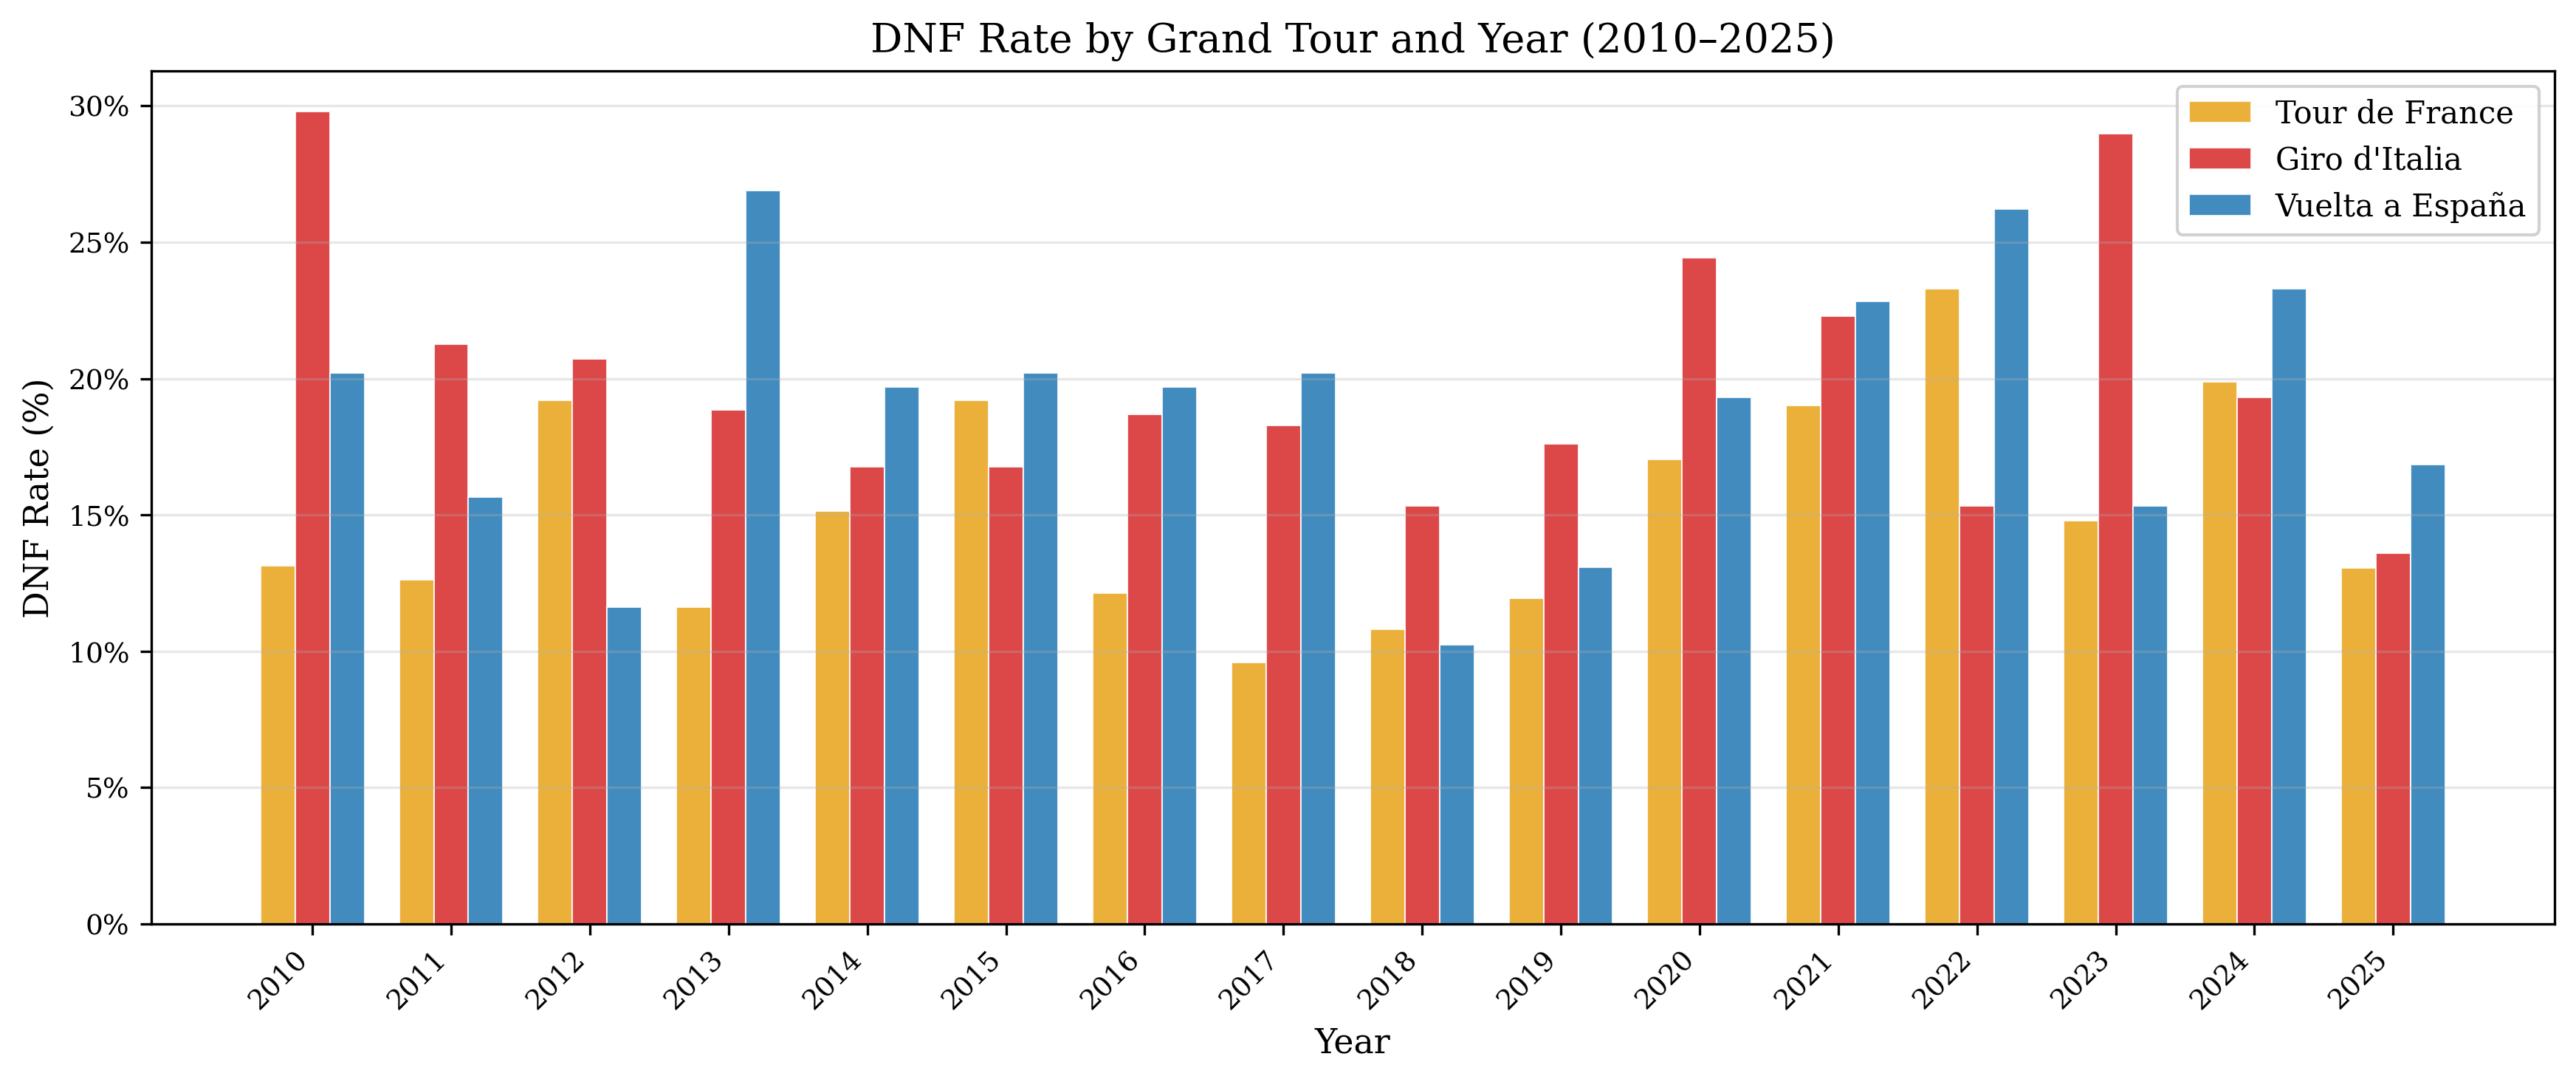
\includegraphics[width=0.5\linewidth]{Afsnit/Billeder/fig2_dnf_rate_by_race_year.png}
    \caption{DNF rate by Grand Tour and year (2010--2025). The Tour de France consistently shows the lowest abandonment rate, while the Giro d'Italia typically shows the highest.}
    \label{fig:dnf_by_year}
\end{figure}

The econometric approach uses Cox proportional hazard models, which model the instantaneous probability of abandonment at each stage conditional on the rider still being in the race. A time-varying extension adds stage-level covariates that change from stage to stage within a race. The main findings are: (i) a rider's historical DNF rate is the strongest predictor of abandonment (HR $= 1.55$, $p < 0.001$); (ii) the Tour de France has significantly lower abandonment hazard than the Vuelta (HR $= 0.865$, $p = 0.002$); and (iii) mountain stages raise daily abandonment hazard (HR $= 1.034$, $p = 0.025$).

The paper is structured as follows. Section~\ref{sec:theory} presents the theoretical framework and reviews relevant literature. Section~\ref{sec:data} describes the data and variables. Section~\ref{sec:empirical_strategy} explains the methodology. Section~\ref{sec:results} presents results. Section~\ref{sec:robustness} provides robustness checks. Section~\ref{sec:discussion} discusses the economic and managerial implications of the findings. Section~\ref{sec:conclusion} concludes with limitations and suggestions for future research.


\newpage

% --------------------------------------------------
% 2. THEORETICAL FRAMEWORK AND LITERATURE
% --------------------------------------------------
\section{Theoretical Framework and Literature Review}
\label{sec:theory}

\subsection{The Economics of Rider Abandonment}

A Grand Tour lasts three weeks and consists of 21 stages. At the start of each stage, every rider still in the race faces a decision: continue or abandon. This paper frames that decision as a rational choice under uncertainty, where the rider and his team compare the expected benefit of continuing (GC position gains, UCI points, sponsor exposure, contract value) against the expected cost (fatigue, injury risk, reduced future performance).

This framing builds on tournament theory as developed by \textcite{rosen1981superstars} and \textcite{lazear1981rank}. Prize structures in tournaments are typically convex: the reward gap between first and second place far exceeds the gap between 50th and 51st. In Grand Tour cycling, this means riders near the top of the GC standings have disproportionately more to gain from staying in the race, while a rider in 80th place may rationally withdraw and save energy for future events. \textcite{szymanski2003economicdesign} provides a broader framework for understanding how the design of sporting contests shapes competitive incentives, and the same logic applies to the stage-by-stage structure of Grand Tours.

A distinctive feature of Grand Tours, compared to the single-contest tournaments in \textcite{lazear1981rank}, is their \emph{nested} or \emph{multi-stage} structure. Each individual stage functions as a tournament (with stage wins and time bonuses as prizes), the 21-stage GC classification is a tournament across stages, and the season-long UCI ranking is a tournament across races. These layers create competing incentive gradients. A domestique may have no stake in the GC tournament but a strong interest in winning an individual stage; a GC contender cares little about individual stage prizes but enormously about the overall classification. This means the same physical event (a mountain stage, for example) generates different economic incentives for different riders depending on which layer of the tournament structure they are competing in.

The multi-stage structure also introduces an \emph{option value} dimension to the continuation decision. At each stage, a rider who is still in the race holds an option: the option to win a future stage, to move up in the GC standings, or to be available for a team strategic move later in the race. Continuing preserves this option; abandoning extinguishes it permanently. The value of the option depends on how many stages remain (higher early in the race), the rider's current position (higher for riders still in GC contention), and the expected difficulty of upcoming stages (lower if brutal mountains lie ahead). This option-value logic predicts that abandonment hazard should increase over the course of a race (as fewer stages remain, the option value of continuing diminishes) and should be higher on mountain stages (which impose a large exercise cost on the option). Both predictions are broadly consistent with the descriptive patterns in the data.

This tournament logic extends to the team level. As discussed in the course lectures on sport clubs as profit-maximising firms (Lecture F2), teams operate with budget constraints and strategic objectives \parencite{blair2012sports}. A team may withdraw a domestique who has fulfilled his support role and is carrying an injury, preserving his physical capital for races where his marginal product will be higher. Conversely, if a GC contender abandons, the domestiques allocated to protect him lose their primary function. The team thus acts as a firm making resource-allocation decisions about its riders, weighing each rider's expected marginal contribution in the current race against his expected contribution in future events.

\subsection{Labour Markets and Contracts in Professional Cycling}

Professional cyclists operate in a labour market that shares features with other professional sports labour markets. \textcite{kahn2000labormarket} argues that professional sports provide a uniquely useful laboratory for studying labour-market questions because of the availability of detailed performance data and the repeated nature of competition. Grand Tour cycling fits this framework: riders produce observable output (stage results, GC rankings, race completions) that signals their quality to teams negotiating future contracts. \textcite{rottenberg1956baseball} established that even in highly regulated sports labour markets, players respond to economic incentives in predictable ways, and the same logic applies to cyclists deciding whether to continue or withdraw.

Within this framework, abandoning a race is a negative performance signal. A rider who does not finish provides less information to the market about his ability, and the act of abandoning may be interpreted as evidence of fragility or insufficient preparation. However, the reputational cost of a DNF depends on context: a domestique who abandons after serving his team leader for two weeks faces different labour-market consequences than a GC contender who abandons while in fifth place (Lectures F4 and F5).

The contract structure in professional cycling adds a further dimension. \textcite{krautmann2002contracts} show that in Major League Baseball, contract length reflects expected future performance and the information environment. In cycling, riders on short-term contracts approaching renewal face different incentives from those on long-term deals. A rider in a contract year may push through pain and fatigue to signal durability, knowing that a DNF could weaken his bargaining position. Conversely, a rider with a secure multi-year contract may abandon more freely, since the immediate reputational cost is buffered by the existing agreement. \textcite{kahn1993freeagency} provides evidence from baseball that the structure of labour-market institutions (free agency, reserve clauses) affects player behaviour, and analogous institutional features in cycling (the transfer system, minimum wage regulations, team licence obligations) shape the incentive environment in which abandonment decisions are made.

The dataset includes each rider's historical DNF rate. This variable can be interpreted in two ways: a high rate may indicate a ``fragile type'' who faces higher continuation costs, or it may reflect that a rider with several past DNFs faces lower marginal reputational cost from one more, because the signal has already been sent. Both interpretations predict a positive association with current abandonment hazard.

Race prestige provides another source of variation. The Tour de France attracts the largest television audiences, the most media coverage, and the most sponsor attention, so the marginal revenue product of continued participation is likely higher in the Tour than in the Giro or Vuelta \parencite{blair2012sports}. This connects to the course material on advertisement and TV rights (Lecture F3): broadcasting revenues and sponsor contracts are tied to participation and visibility, giving riders and teams stronger incentives to persist in higher-prestige events. \textcite{mignot2016cycling} documents the Tour's dominant commercial position among Grand Tours, providing historical context for this incentive asymmetry.

\subsection{Related Empirical Work}

Several studies in sports economics have used hazard or duration models to analyse decisions with a structure similar to rider abandonment. The course material on managers, coaches, and team performance (Lecture F6) discusses how managerial tenure in football can be modelled as a survival process, where dismissal probability depends on match results, league position, and club characteristics. The underlying logic is the same as in this paper: an event (dismissal or abandonment) occurs at some point during a spell (a season or a race), and covariates shift the probability of that event. \textcite{boeri2008italianjob} study career concerns among referees in Italian football and show how incentive structures lead to strategic behaviour that can be inferred from patterns in the data, an approach conceptually similar to what this paper does with rider-level proxies. \textcite{rosen2001labourmarkets} provide a broader treatment of how professional sports labour markets generate observable signals that researchers can exploit.

The survival-analysis methodology used in this paper has parallels in other sports contexts. Career-duration studies in American football, baseball, and basketball use hazard models to estimate the determinants of career length, treating retirement or release as the event of interest. The distinguishing feature of the present application is that the ``spell'' is a single race (21 stages) rather than an entire career, which gives much finer temporal resolution and allows stage-level covariates that vary within the spell. \textcite{courty2003ticketresale} demonstrates from a different angle that outcomes within sporting events carry economic value: his work on ticket resale shows that spectators pay a premium for uncertainty of outcome, and rider abandonment resolves that uncertainty, reducing the entertainment and therefore commercial value of remaining stages.

Outside the course material, there is a growing literature on cycling economics \parencite{torgler2007cycling}, but most of it focuses on doping, team strategy, or stage-win determinants. Very few papers model within-race attrition from an explicitly economic perspective. This is surprising, because Grand Tours generate rich stage-by-stage panel data well suited to survival analysis, and because abandonment has clear economic consequences: it reshuffles GC standings, redistributes prize money and UCI points, and affects the information content of race results as signals of rider quality. This paper aims to fill that gap by applying a standard econometric framework to a novel dataset, and by interpreting the results through the lens of tournament incentives and labour-market signalling.


\newpage

% % --------------------------------------------------
% % 3. DATA
% % --------------------------------------------------
% \section{Data}

% \subsection{Data Collection}
% \begin{itemize}
%     \item Describe the web-scraping pipeline: stage-by-stage results, rider profiles, and stage metadata from ProCyclingStats for all three Grand Tours from 2010 to 2025 (Script 01).
%     \item Explain the feature-engineering process: construction of the rider-race panel with survival time (number of stages completed) and event indicator (1 = abandoned), plus rider-level and stage-level covariates (Script 02).
% \end{itemize}

% \subsection{Variable Definitions and Economic Interpretation}
% \begin{itemize}
%     \item Present each variable with its economic proxy interpretation:
%     \begin{itemize}
%         \item \textbf{GC contender} $\rightarrow$ tournament incentive proxy (expected returns from continued participation).
%         \item \textbf{Race dummies} (Tour de France, Giro) $\rightarrow$ event-value proxy (media exposure, sponsor visibility, marginal revenue product).
%         \item \textbf{Previous DNF rate} $\rightarrow$ rider-specific expected continuation cost / revealed risk type.
%         \item \textbf{Mountain stage, distance} $\rightarrow$ marginal cost of effort (time-varying).
%         \item \textbf{Age, experience} $\rightarrow$ human capital and durability.
%         \item \textbf{Team size, team average age} $\rightarrow$ team-resource controls.
%     \end{itemize}
% \end{itemize}

% \subsection{Summary Statistics}
% \begin{itemize}
%     \item Present Table~1 (summary statistics): 9{,}045 rider-race observations; 18\% abandonment rate; average survival time of 19.2 stages; mean age 29; 15.4\% classified as GC contenders.
%     \item Discuss the roughly equal split across the three Grand Tours ($\approx$3{,}000 each).
%     \item Include Figure~1 (Kaplan--Meier survival curves by Grand Tour) and Figure~2 (DNF rate by race and year) and briefly describe the patterns.
% \end{itemize}

% --------------------------------------------------
% 3. DATA
% --------------------------------------------------
\section{Data}
\label{sec:data}

\subsection{Data Collection}

The dataset used in this paper was constructed by scraping stage-by-stage results, rider profiles, and stage metadata from ProCyclingStats, a widely used public database for professional cycling statistics. The scraping covers all editions of the three Grand Tours (the Tour de France, the Giro d'Italia, and the Vuelta a Espa\~{n}a) from 2010 to 2025, giving 16 years and 48 race editions in total. The raw data collection produced three files: a rider-stage results file with one row per rider per stage (recording the rider's finishing position, time, and whether they abandoned), a rider profiles file with biographical information (date of birth, nationality, height, weight), and a stage metadata file with information about each stage (distance, stage type, date).

The raw data were then cleaned and transformed into two analysis-ready datasets. The first is a rider-race panel with one row per rider per race edition. For each observation, the key outcome variables are the \emph{survival time} (defined as the number of stages the rider completed before either finishing the race or abandoning) and an \emph{event indicator} that equals 1 if the rider abandoned (DNF, DNS, DSQ, or OTL) and 0 if the rider finished all 21 stages. Riders who finish the race are treated as right-censored observations in the survival model: we know they survived the full duration, but we do not observe the counterfactual stage at which they would have abandoned. The second dataset is a time-varying panel with one row per rider per stage interval, structured in the start-stop format required for time-varying Cox models. This dataset allows stage-level covariates such as stage type and distance to vary within a race.

\subsection{Variable Definitions and Economic Interpretation}

Table~\ref{tab:variables} in the Appendix provides a full overview of variables and their economic interpretations. Importantly, none are direct financial measures; the dataset does not contain prize money, rider salaries, or team budgets. Instead, the variables are interpreted as proxies for the underlying economic forces described in the theoretical framework, a common approach when financial data is unavailable \parencite{kahn2000labormarket}.

The key variables are: a GC contender indicator (equal to 1 if the rider finished in the top 20 of any Grand Tour GC in the two preceding years, capturing tournament incentives); the historical DNF rate (the share of prior Grand Tour starts ending in abandonment, capturing rider-specific continuation costs); race dummies for the Tour de France and Giro d'Italia with the Vuelta as baseline (proxying event value through media, sponsor, and UCI point differences); and in the time-varying model, stage-type dummies and standardised distance (proxying the marginal cost of effort). Controls include rider age, experience, team size, team average age, and a centred year trend. All backward-looking variables are computed using only pre-race information to avoid endogeneity.

\subsection{Summary Statistics}

Table~\ref{tab:summary} presents the summary statistics for the main rider-race panel. The dataset contains 9{,}045 rider-race observations, distributed almost equally across the three Grand Tours: 3{,}008 in the Tour de France, 3{,}023 in the Giro d'Italia, and 3{,}014 in the Vuelta a Espa\~{n}a. The overall abandonment rate is 18\%, meaning that roughly one in five riders who start a Grand Tour does not finish. The median survival time is 21 stages (i.e.\ the full race), reflecting the fact that most riders do finish, but the mean is 19.2 stages, pulled down by those who abandon earlier.

\begin{table}[htbp]
\centering
\caption{Summary statistics for the rider-race panel (2010--2025).}
\label{tab:summary}
\small
\begin{tabular}{lrrrrrr}
\toprule
Variable & N & Mean & SD & Min & Median & Max \\
\midrule
DNF (1 = abandoned)          & 9{,}045 & 0.180 & 0.384 & 0 & 0 & 1 \\
Survival time (stages)       & 9{,}045 & 19.15 & 4.222 & 0 & 21 & 21 \\
Age at race start            & 8{,}939 & 28.97 & 4.179 & 20 & 29 & 43 \\
Previous Grand Tours started & 9{,}045 & 4.254 & 4.312 & 0 & 3 & 25 \\
Historical DNF rate          & 9{,}045 & 0.135 & 0.226 & 0 & 0 & 1 \\
GC contender (0/1)           & 9{,}045 & 0.154 & 0.361 & 0 & 0 & 1 \\
Team size                    & 9{,}045 & 8.523 & 0.501 & 7 & 9 & 9 \\
Team average age             & 9{,}045 & 28.98 & 1.696 & 23.0 & 28.9 & 33.6 \\
\midrule
Race: Tour de France         & 3{,}008 & & & & & \\
Race: Giro d'Italia          & 3{,}023 & & & & & \\
Race: Vuelta a Espa\~{n}a    & 3{,}014 & & & & & \\
\bottomrule
\end{tabular}
\end{table}

The riders have a mean age of about 29 years and have started an average of 4.3 Grand Tours before the current one. The mean historical DNF rate is 0.135, but the median is 0, indicating that many riders have never abandoned before. About 15.4\% of observations involve a GC contender. Team size has very little variation (most teams start with 8 or 9 riders, as dictated by race regulations).

Figure~\ref{fig:km_curves} shows Kaplan--Meier survival curves by Grand Tour. Two patterns stand out. First, the Tour de France curve lies consistently above the other two: by the final stage, roughly 85\% of Tour starters are still racing, compared to about 80\% in the Giro and 81\% in the Vuelta. Second, all three curves show a steady, approximately linear decline rather than a sharp drop at any particular stage, suggesting that abandonment is spread across the race. Both patterns are consistent with the economic framework: the Tour's higher survival rate fits the incentive interpretation, and the gradual decline fits a model where riders continually reassess the cost-benefit balance.

\begin{figure}[H]
    \centering
    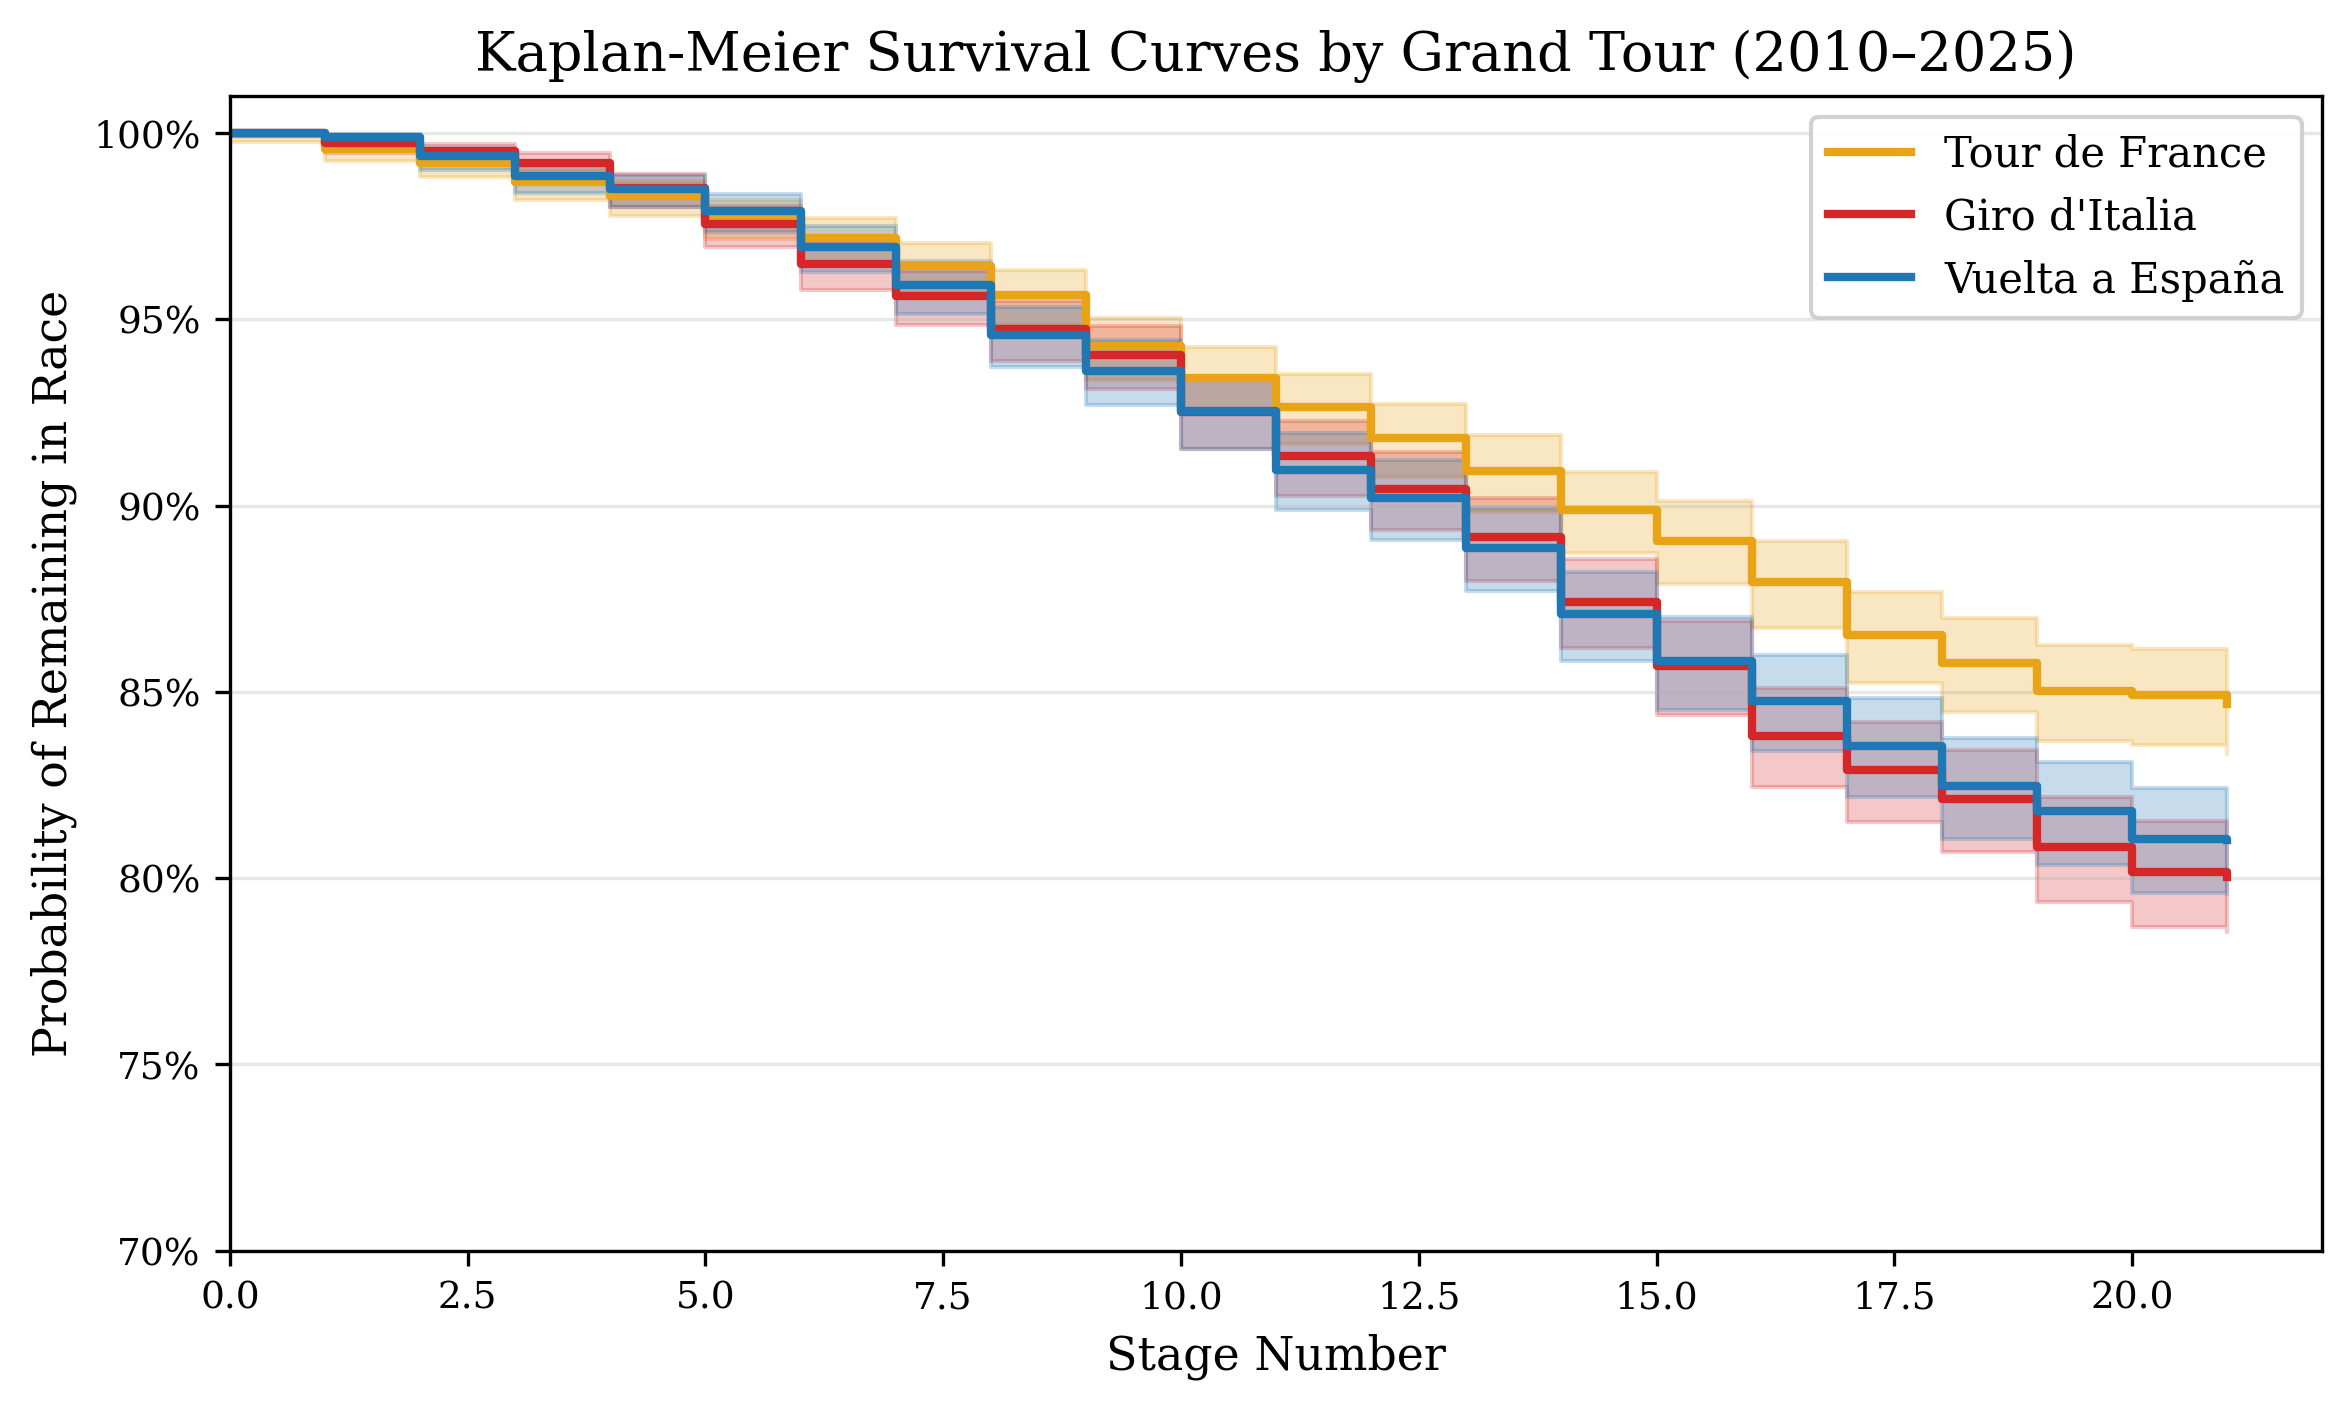
\includegraphics[width=0.6\linewidth]{Afsnit/Billeder/fig1_km_curves.png}
    \caption{Kaplan--Meier survival curves by Grand Tour (2010--2025). The curves show the estimated probability that a rider is still in the race at each stage number, separately for the Tour de France, Giro d'Italia, and Vuelta a Espa\~{n}a. The Tour de France curve lies consistently above the other two, indicating higher survival rates at every stage.}
    \label{fig:km_curves}
\end{figure}

Figure~\ref{fig:dnf_by_year}, already shown in the introduction, adds a temporal dimension: DNF rates fluctuate year to year, but the Tour de France is consistently at or near the bottom. The persistent gap between races points toward a structural difference that the econometric models will capture through the race dummies.
\newpage

% --------------------------------------------------
% 4. EMPIRICAL STRATEGY
% --------------------------------------------------
\section{Empirical Strategy}
\label{sec:empirical_strategy}

\subsection{Cox Proportional Hazard Model}

The central methodological choice is the Cox proportional hazard (PH) model \parencite{cox1972regression, cleves2010survival}, implemented using the \texttt{lifelines} library for Python \parencite{davidson2023lifelines}. The model is well suited to the data for three reasons. First, it is semi-parametric: it does not require a parametric assumption about the shape of the baseline hazard, which matters because there is no strong prior about whether abandonment risk follows a Weibull or exponential distribution over stages. Second, the Cox model naturally handles right-censoring: riders who complete all 21 stages are correctly accounted for as observations where the event did not occur. Third, the model captures duration dependence through the shared baseline hazard, allowing abandonment risk to evolve across stages without imposing a functional form.

The hazard function for rider $i$ at stage $t$ is:
\begin{equation}
    h(t \mid \mathbf{X}_i) = h_0(t) \exp\!\left(\mathbf{X}_i \boldsymbol{\beta}\right),
\end{equation}
where $h_0(t)$ is the unspecified baseline hazard, $\mathbf{X}_i$ is a vector of covariates, and $\boldsymbol{\beta}$ is the vector of log-hazard coefficients. The hazard ratio $\exp(\beta_k)$ is the key quantity: values above 1 indicate higher abandonment risk, values below 1 indicate a protective effect.

The basic model includes: rider age and previous Grand Tour starts (human capital proxies), historical DNF rate (continuation cost proxy), a GC contender indicator (tournament incentive proxy), team size and team average age (team-resource controls), race dummies for the Tour de France and Giro d'Italia with the Vuelta as baseline (event-value proxies), and a centred year trend.

\subsection{Time-Varying Extension}

A limitation of the basic model is that it assigns fixed covariate values for the entire race, but stage difficulty changes day by day. To address this, a time-varying Cox model adds four stage-type dummies (mountain, hilly, individual time trial, team time trial; flat as baseline) and standardised stage distance. These covariates are entered in the counting-process (start-stop) format, where each row represents one stage interval for one rider \parencite{cleves2010survival}. This permits a direct test of whether stage-level physical costs affect abandonment independently of rider-level characteristics.

\subsection{Proportional Hazards Assumption}

Both models rest on the proportional hazards assumption: the hazard ratio between any two riders is constant over time. This is tested using Schoenfeld residuals \parencite{schoenfeld1982residuals}. Table~\ref{tab:schoenfeld} in the Appendix reports the test statistics: no covariate is significant at the 5\% level, providing no evidence against the assumption. The Schoenfeld residual plots (Figure~\ref{fig:schoenfeld} in the Appendix) confirm visually that there is no systematic trend over time.

\newpage
% --------------------------------------------------
% 5. RESULTS
% --------------------------------------------------
\section{Results}
\label{sec:results}

\subsection{Basic Cox Model}

Table~\ref{tab:cox_basic} reports the estimated hazard ratios from the basic Cox PH model. Of the nine covariates included, two are statistically significant at the 1\% level and one at the 5\% level. The remaining six covariates, including age, experience, team controls, the Giro d'Italia dummy, and the year trend, are not statistically distinguishable from zero.

\begin{table}[H]
\centering
\caption{Basic Cox proportional hazard model. The outcome is rider abandonment. Hazard ratios above 1 indicate higher abandonment risk; below 1 indicate lower risk. Significance: *** $p<0.001$, ** $p<0.01$.}
\label{tab:cox_basic}
\small
\renewcommand{\arraystretch}{1.3}
\begin{tabular}{@{} lrrrr @{}}
\toprule
Variable & Hazard Ratio & 95\% CI & $p$-value & \\
\midrule
Age                 & 0.998 & [0.988, 1.009] & 0.736 & \\
Experience          & 1.004 & [0.994, 1.015] & 0.424 & \\
Previous DNF rate   & 1.549 & [1.316, 1.822] & $<$0.001 & *** \\
GC contender        & 1.156 & [1.040, 1.286] & 0.008 & ** \\
Team size           & 0.992 & [0.903, 1.090] & 0.872 & \\
Team average age    & 0.987 & [0.963, 1.011] & 0.291 & \\
Tour de France      & 0.865 & [0.790, 0.946] & 0.002 & ** \\
Giro d'Italia       & 1.065 & [0.977, 1.161] & 0.150 & \\
Year (centred)      & 0.999 & [0.989, 1.009] & 0.836 & \\
\bottomrule
\multicolumn{5}{l}{\footnotesize Baseline race: Vuelta a Espa\~{n}a. $N = 9{,}045$ rider-race observations.}
\end{tabular}
\end{table}

The strongest predictor is the previous DNF rate (HR $= 1.549$, $p < 0.001$), implying that a rider who has always abandoned faces roughly 55\% higher hazard than one who has never abandoned.\footnote{The coefficient is reported per unit (0\% to 100\% historical DNF rate). For a one-SD increase ($\approx$22.6 pp), the effect is approximately $1.549^{0.226} \approx 1.10$.} This is consistent with two complementary interpretations: past abandonment reveals a ``fragile type'' with higher expected continuation costs, and from a signalling perspective \parencite{kahn2000labormarket}, a high DNF rate is a negative performance signal that may reflect career-stage dynamics.

The GC contender dummy (HR $= 1.156$, $p = 0.008$) indicates approximately 16\% higher abandonment hazard for GC contenders. Although seemingly counterintuitive, this is reconcilable with the incentive framework: GC contenders ride near their physiological ceiling and are more vulnerable to accumulated fatigue, and teams may strategically withdraw GC contenders who have fallen out of contention to preserve them for future races. In the tournament theory framework of \textcite{lazear1981rank}, the expected prize diminishes sharply once a contender falls too far behind the leader, making exit the rational response.

The Tour de France dummy (HR $= 0.865$, $p = 0.002$) implies roughly 14\% lower abandonment hazard than the Vuelta. This is consistent with the event-value hypothesis: the Tour offers higher prize money, greater media coverage, and more UCI ranking points, raising the economic returns from continued participation. This connects to the media economics framework in the course material (Lecture F3): broadcasting revenues and sponsor contracts are tied to participation and visibility \parencite{blair2012sports}. The Giro d'Italia coefficient is positive but not significant. The insignificance of age, experience, and team controls suggests these do not independently predict abandonment once DNF history and GC status are accounted for. Figure~\ref{fig:hazard_ratios} in the Appendix displays the hazard ratios in a forest plot.

\subsection{Time-Varying Cox Model}

Table~\ref{tab:cox_timevarying} extends the basic model by adding stage-level covariates that vary within a race.

\begin{table}[H]
\centering
\caption{Time-varying Cox proportional hazard model. Stage-type dummies and standardised distance are entered as time-varying covariates. Significance: * $p<0.05$, $\dagger$ $p=0.05$.}
\label{tab:cox_timevarying}
\small
\renewcommand{\arraystretch}{1.3}
\begin{tabular}{@{} lrrrr @{}}
\toprule
Variable & Hazard Ratio & 95\% CI & $p$-value & \\
\midrule
Age                 & 1.000 & [0.996, 1.003] & 0.923 & \\
Experience          & 1.000 & [0.997, 1.004] & 0.814 & \\
Previous DNF rate   & 1.067 & [1.000, 1.137] & 0.050 & $\dagger$ \\
GC contender        & 1.020 & [0.980, 1.061] & 0.341 & \\
Team size           & 1.000 & [0.972, 1.029] & 0.995 & \\
Tour de France      & 0.981 & [0.951, 1.011] & 0.215 & \\
Giro d'Italia       & 1.015 & [0.985, 1.047] & 0.335 & \\
Year (centred)      & 1.000 & [0.997, 1.003] & 0.943 & \\
Stage: hilly        & 0.997 & [0.964, 1.032] & 0.885 & \\
Stage: mountain     & 1.034 & [1.004, 1.064] & 0.025 & * \\
Stage: indiv.\ TT   & 0.965 & [0.915, 1.019] & 0.198 & \\
Stage: team TT      & 0.965 & [0.879, 1.059] & 0.454 & \\
Distance (z)        & 1.012 & [0.997, 1.027] & 0.111 & \\
\bottomrule
\multicolumn{5}{l}{\footnotesize Baseline stage type: flat. Baseline race: Vuelta a Espa\~{n}a.}
\end{tabular}
\end{table}

Mountain stages are the only stage type that significantly predicts abandonment (HR $= 1.034$, $p = 0.025$), consistent with a marginal-cost-of-effort interpretation: mountain stages impose higher physical demands and raise the instantaneous probability of abandonment on that day.

Once stage-type controls are included, several rider-level predictors lose significance. The GC contender dummy falls from HR $= 1.156$ ($p = 0.008$) to HR $= 1.020$ ($p = 0.341$), and the Tour de France dummy from HR $= 0.865$ ($p = 0.002$) to HR $= 0.981$ ($p = 0.215$). This suggests that part of what the basic model attributed to race identity and rider type was actually the correlation between these variables and stage-level difficulty. The previous DNF rate shrinks to HR $= 1.067$ (marginally significant at $p = 0.050$), partly because the time-varying model estimates effects on the daily rather than race-level hazard.

Taken together, the two models tell a consistent story. Riders with higher historical DNF rates face elevated abandonment hazard, consistent with higher expected continuation costs. The Tour de France generates lower abandonment, consistent with higher incentives from event value. Mountain stages raise the marginal cost of continuation on a given day. Because no direct financial variables are observed, these results should be read as suggestive evidence that economic incentives and costs shape abandonment patterns, not as a definitive causal decomposition.


\newpage

% --------------------------------------------------
% 6. ROBUSTNESS CHECKS
% --------------------------------------------------
\section{Robustness Checks}
\label{sec:robustness}

\subsection{Sub-sample Analysis: GC Contenders and Non-GC Riders}

A natural concern with the pooled model is that the determinants of abandonment may differ between GC contenders and the rest of the field. To investigate this, separate Cox PH models are estimated for GC contenders ($n = 1{,}395$) and non-GC riders ($n = 7{,}650$). The full regression tables are reported in Tables~\ref{tab:cox_gc} and~\ref{tab:cox_nonGC} in the Appendix; here the key findings are summarised.

The previous DNF rate effect is substantially larger for GC contenders (HR $= 2.280$, $p = 0.001$) than for non-GC riders (HR $= 1.472$, $p < 0.001$), and the confidence intervals barely overlap, suggesting meaningful heterogeneity. This is consistent with a higher-stakes signalling environment for GC contenders: a rider whose past abandonment record has already signalled fragility faces compounding reputational and physical costs. In tournament theory terms \parencite{rosen1981superstars, lazear1981rank}, the amplified effect may also reflect the sharper incentive cliff that GC contenders face once they fall out of contention.

The Tour de France protective effect is significant only for non-GC riders (HR $= 0.866$, $p = 0.005$), not for GC contenders (HR $= 0.863$, $p = 0.177$). Although the point estimates are nearly identical, the GC estimate loses precision due to the smaller sub-sample. The pattern suggests that event-value incentives operate primarily through domestiques and support riders, for whom finishing the Tour carries direct benefits in team bonuses, sponsor visibility, and reputational value. GC contenders face a more binary decision: continue if competitive, withdraw if not, regardless of which Grand Tour they are racing.

Economically, this heterogeneity has implications for how we interpret the pooled model. The pooled GC contender coefficient (HR $= 1.156$) is a weighted average of two distinct behavioural regimes: one in which GC contenders are driven by tournament incentives and physical exposure, and one in which non-GC riders respond to event-value gradients. Pooling conceals the fact that the economic forces operating on these two groups are qualitatively different, not just quantitatively. This suggests that future work modelling abandonment should allow for interaction effects between rider role and race-level incentives, rather than assuming a single set of coefficients applies to all riders. The sub-sample results also reinforce the practical value of the analysis for team management: a team selecting riders for a Grand Tour roster should weight a GC candidate's abandonment history more heavily than a domestique's, because the predictive power of past DNF behaviour is substantially stronger for the former group.

%\newpage

%\newpage

%\newpage

\newpage

%Litteraturliste
\renewcommand{\bibname}{Bibliography}
\printbibliography
\newpage

\end{document}